\section{Diagnosing GRPO's Staleness Tolerance}
\label{sec:diagnosis}

We pursue large-$\mu$ training because it offers a compelling promise: accelerating training through extensive data reuse, turning rollout staleness from a constraint into a source of efficiency. Doing so, however, requires understanding when stale rollouts remain useful and when they become destabilizing. Rather than treating high staleness as uniformly harmful, we show that stale rollouts contain exploitable learning signal whose failure mode is localized to a specific class of off-support negative updates. This section identifies why naive high-staleness GRPO breaks (\cref{subsec:clipping_dilemma}), then identify low-ratio negative-advantage
tokens as collapse triggers (\cref{subsec:negative_drift}), and finally localize
the destabilizing updates to the post-trigger suffix
(\cref{subsec:localizing_harmful_updates}).




% \begin{figure*}[tbh]
%     \centering
%     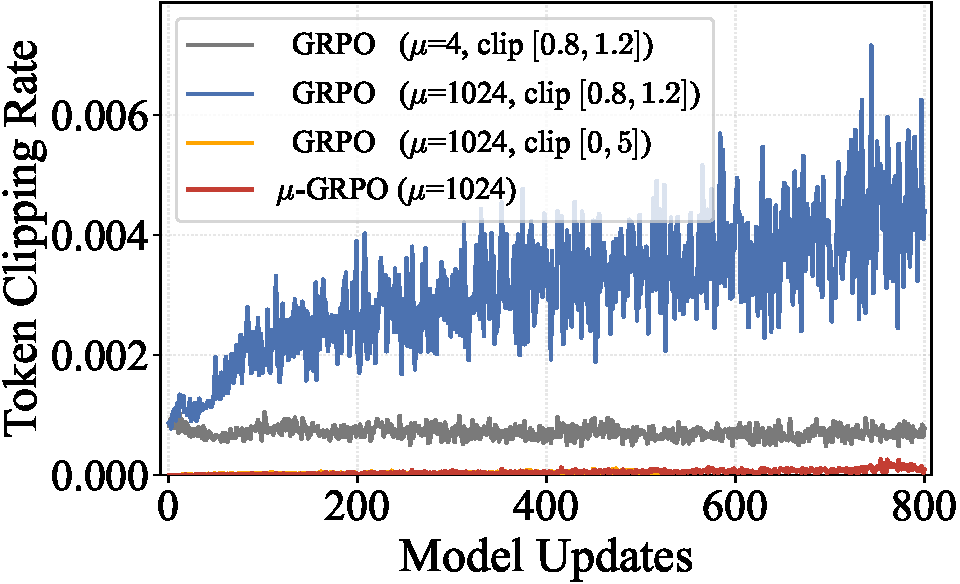
\includegraphics[width=0.48\textwidth]{figures/token_clipping.pdf}
%     \hfill
%     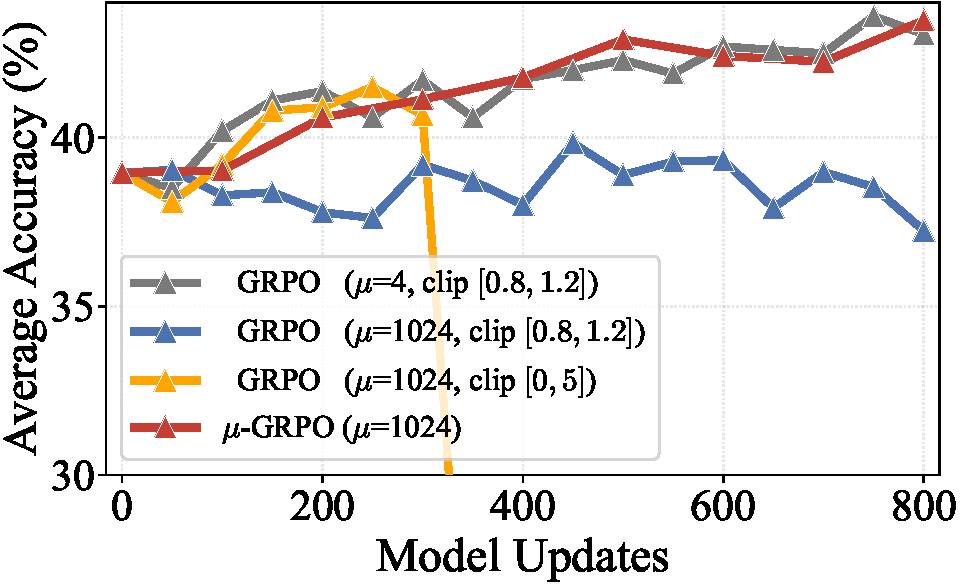
\includegraphics[width=0.48\textwidth]{figures/performance_comparison.pdf}
%     \caption{
%     \textbf{Training stability and performance of GRPO variants and \boldmath \ourmethod.}
%     (\textit{Left}) Token clipping ratio dynamics during training.
%      Large-$\mu$ GRPO with clipping exhibits a growing clipping rate, while \ourmethod\ keeps clipping near zero.
%     (\textit{Right}) Average accuracy over five math benchmarks. Relaxed clipping improves early learning but becomes unstable, whereas \(\mu\)-GRPO maintains stable training and achieves the best final accuracy. Experiments are conducted on Qwen-2.5-Math-7B.}
    
%     \label{fig:grpo_clipping_and_performance}
% \vspace{-1em}

% \end{figure*}

\begin{wrapfigure}{r}{0.65\textwidth}
\vspace{-1.0em}
\centering
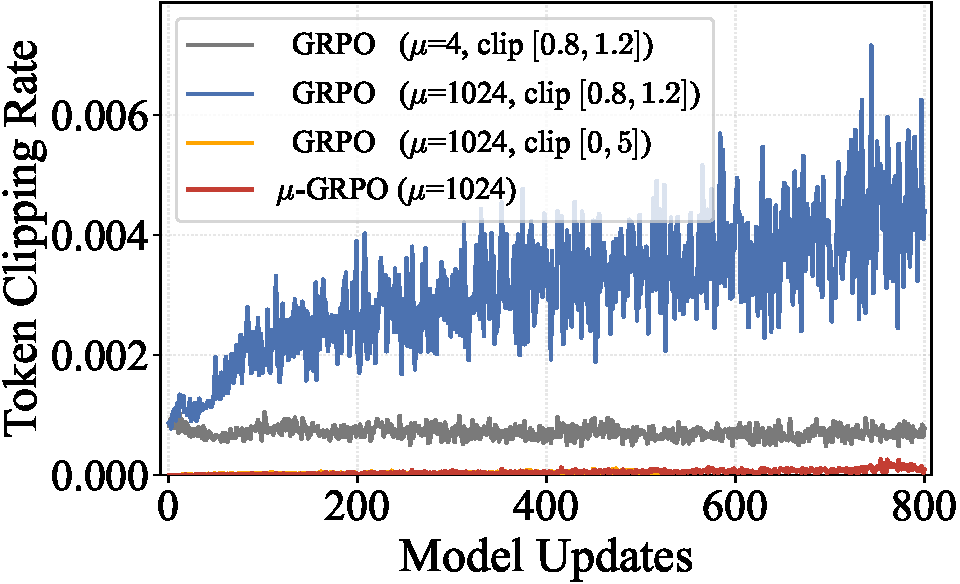
\includegraphics[width=0.32\textwidth]{figures/token_clipping.pdf}
\hfill
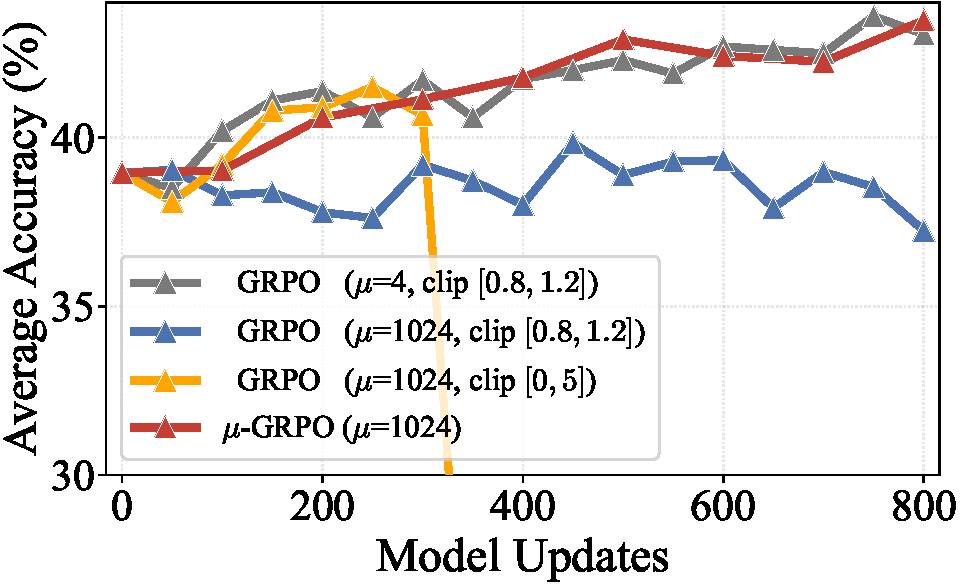
\includegraphics[width=0.32\textwidth]{figures/performance_comparison.pdf}
\vspace{-1.5em}
\caption{\textbf{Clipping creates a high-staleness dilemma.}
At $\mu=1024$, $[0.8,1.2]$ bound clips many more tokens and plateaus at lower accuracy ({\color{plotblue}blue}), while relaxed clipping recovers early gains but later collapses ({\color{plotyellow}yellow}).
Results are on Qwen2.5-Math-7B.}
\label{fig:grpo_clipping_and_performance}
\vspace{-1em}
\end{wrapfigure}


\subsection{The Clipping Dilemma under High Staleness}
\label{subsec:clipping_dilemma}

% Under low staleness, the behavior policy $\beta$ and current policy
% $\pi_\theta$ remain close, so the standard interval $[0.8,1.2]$ clips only a
% small fraction of tokens. Under a large $\mu\,=\,1024$, the same behavior policy is reused
% for many consecutive updates. As $\pi_\theta$ drifts from $\beta$, more rollout
% tokens fall outside this interval and are clipped to constants, contributing no gradient. Figure~\ref{fig:grpo_clipping_and_performance} shows the resulting dilemma. The standard bound run of $[0.8,1.2]$ has a substantially higher and increasing token
% clipping rate (Figure~\ref{fig:grpo_clipping_and_performance} (left), and its accuracy plateaus at a lower level (Figure~\ref{fig:grpo_clipping_and_performance} (right). Relaxing the clipping range to
% $[0,5]$ recovers strong early learning, showing that
% stale rollouts still contain useful gradient signal. However, relaxed clipping
% alone is unstable: after an initial improvement phase, the run collapses
% mid-training. Thus, the challenge in high-staleness GRPO is not simply
% whether stale rollouts are useful, but how to expose their learning signal
% without activating the destabilizing updates that emerge as the policy drifts
% away from the behavior distribution.

Under low staleness, the behavior policy $\beta$ and current policy $\pi_\theta$ remain close, so the standard $[0.8,1.2]$ interval clips only outlying updates.
Under high staleness, however, rollouts sampled from the same $\beta$ are reused for many updates, causing the current policy $\pi_\theta$ to drift away from the rollout distribution. We study this clipping dilemma at a high staleness $\mu=1024$ in Figure~\ref{fig:grpo_clipping_and_performance}. With the standard clipping bound $[0.8,1.2]$, an increasing fraction of rollout tokens fall outside the interval and are clipped, suppressing their gradient contribution (Figure~\ref{fig:grpo_clipping_and_performance}, left). As a result, the run plateaus at a lower accuracy (Figure~\ref{fig:grpo_clipping_and_performance}, right). In contrast, relaxing the clipping range to $[0,5]$ keeps the clipping ratio low and recovers strong early learning, indicating that stale rollouts still contain useful gradient signal. However, this signal is not continuously safe to use: after the initial improvement phase, the relaxed-clipping run collapses mid-training.
These results show that high-staleness GRPO is limited not by the absence of useful signal in stale rollouts, but by the difficulty of exposing that signal while suppressing destabilizing updates as $\pi_\theta$ drifts away from the behavior policy $\beta$.

\subsection{Negative-Advantage Drift as a Collapse Signal}
\label{subsec:negative_drift}

The clipping dilemma in Figure~\ref{fig:grpo_clipping_and_performance}
shows that neither extreme is satisfactory under high staleness. Tight clipping
is stable but clips away much of the stale rollout signal, limiting learning.
Relaxed clipping exposes this signal and enables strong early improvement, but
eventually collapses. We therefore ask which part of the relaxed update becomes
dangerous.

We focus on negative-advantage tokens. For GRPO, a negative advantage
means that the response scored worse than other responses in the same group, so
the update decreases the probability of the tokens that produced it. Under high
staleness, many successive updates use rollouts from the same frozen behavior
policy $\beta$. With relaxed clipping, the policy can therefore repeatedly
suppress negative-advantage actions sampled from this fixed distribution.

This repeated suppression creates a simple diagnostic. The importance ratio
$\rho_t=\pi_\theta(a_t\mid s_t)/\beta(a_t\mid s_t)$ compares how likely a token
is under the current policy and under the behavior policy that generated it. A
small ratio on negative-advantage tokens means that actions once plausible under
$\beta$ have become much less likely under $\pi_\theta$. The blue and gray lines in Figure~\ref{fig:nav_explanation} 
show that this is exactly what happens in collapsed runs:
$\mathbb{E}[\rho_t\mid A_t<0]$ drops sharply, while stable runs keep it close to
one. Collapse is therefore preceded by the over-suppression of low-reward behavior-sampled responses.

Formally, for a response $y$\,$=$\,$(a_1,\ldots,a_T)$, we omit the response index $i$.
With the relaxed clipping range $[0,5]$, the effective gradient for a
negative-advantage token is
$
    \nabla_\theta \ell_t(\theta)
    =
    |A_t|\,\rho_t(\theta)
    \nabla_\theta \log \pi_\theta(a_t\,|\, s_t).
$
Thus, relaxed clipping allows negative-advantage updates to keep suppressing
behavior-sampled actions over a much wider ratio range.

This motivates using low-ratio negative-advantage tokens as collapse triggers.
Prior work on training--inference mismatch similarly captures low-ratio events to
mask out unstable updates~\cite{liu-li-2025-rl-collapse}. Here, we treat such events
as boundaries where useful stale learning begins to turn into destructive policy
drift, and then ask which subsequent updates must be masked to prevent collapse.


% \subsection{Negative-Advantage Drift as a Collapse Signal}
% \label{subsec:negative_drift}

% The clipping dilemma shows that stale rollouts can provide useful gradients, but also that exposing these gradients with relaxed clipping introduces a distinct instability. So we ask which part of the relaxed update is responsible for this collapse. To localize the failure, we inspect importance-ratio dynamics by
% advantage sign. The diagnostic statistic in Figure~\ref{fig:nav_explanation} is
% the mean importance ratio over negative-advantage tokens,
% $\mathbb{E}[\rho_t \,|\, A_t<0]$. In collapsed runs, this statistic
% drops sharply before collapse, whereas stable runs keep it close to one.

% For notation, we omit the response index from
% Section~\ref{sec:preliminaries}: for a response
% $y=(a_1,\ldots,a_T)$, write $\rho_t=\rho_{i,t}$ and let $A_t=A_i$ be the
% response-level advantage assigned to token $t$. Under the relaxed range $[0,5]$,
% the effective gradient for a negative-advantage token is
% \begin{equation}
%     \nabla_\theta \ell_t(\theta)
%     =
%     |A_t|\,\rho_t(\theta)
%     \nabla_\theta \log \pi_\theta(a_t\mid s_t).
%     \label{eq:negative_grad}
% \end{equation}
% Thus negative-advantage updates decrease the probability of behavior-sampled
% actions. On fresh or mildly stale data, this is the intended signal for
% suppressing low-reward responses. Under large staleness, however, all
% minibatches in a stage are drawn from the same frozen behavior distribution
% $\beta$. Even though each response may be used only once, successive updates
% repeatedly push down negative-advantage actions from the same behavior-support
% region while $\beta$ remains fixed. As $\pi_\theta$ drifts away from this
% region, later negative-advantage responses can be evaluated on increasingly
% off-support prefixes. A very small ratio is therefore a practical boundary
% signal.

% Prior work on training-inference mismatch uses low-ratio events to trigger
% masking of unstable updates~\cite{liu-li-2025-rl-collapse}. Building on this
% idea, we use low-ratio negative-advantage tokens as boundary triggers, but treat
% the masking scope as an empirical and mechanistic question: once such a trigger
% fires, which subsequent updates must be removed to prevent collapse?

\begin{figure*}[!t]
    \centering
    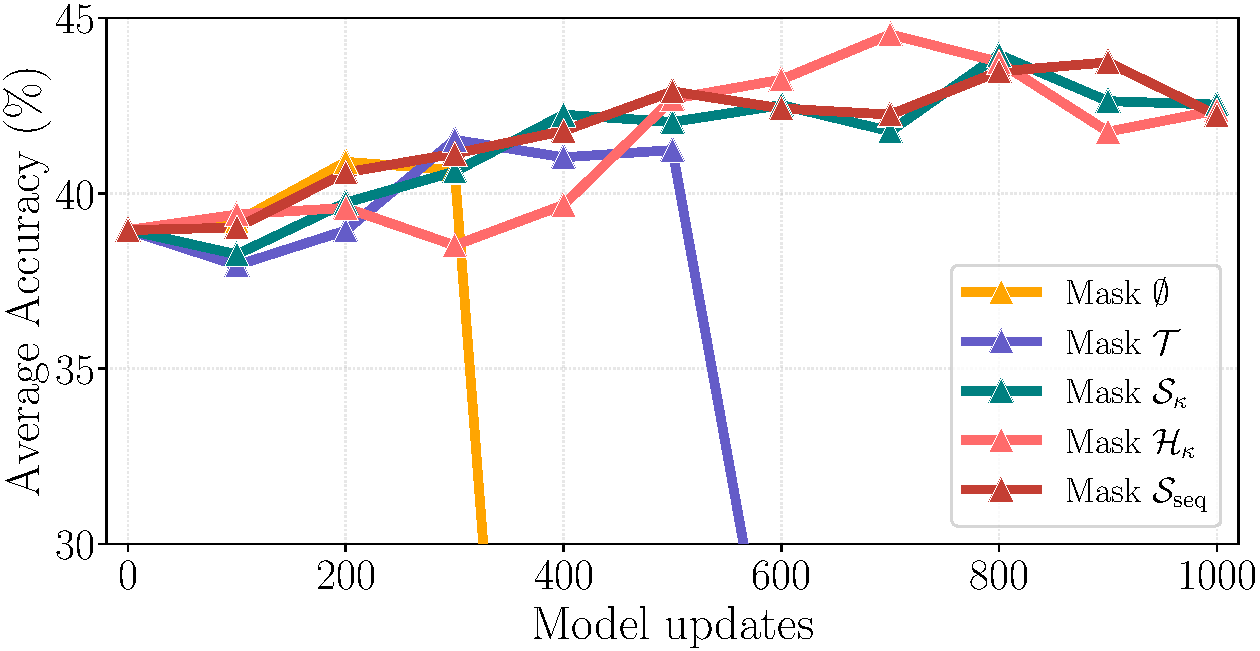
\includegraphics[width=0.49\textwidth]{figures/nav_explanation.pdf}
    \hfill
    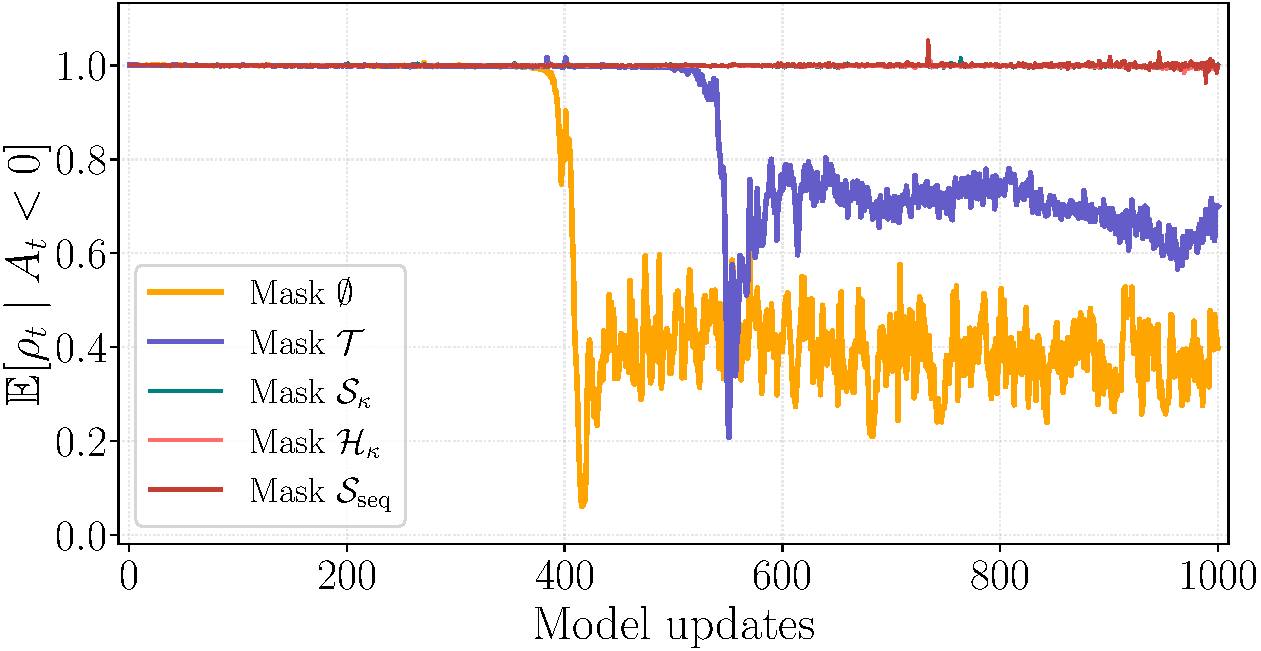
\includegraphics[width=0.49\textwidth]{figures/nav_explanation_ratio_mean_neg.pdf}
\caption{
\textbf{Localizing the harmful updates.}
Under relaxed clipping $[0,5]$, masking only trigger tokens $\mathcal T$ still
collapses, while masking the non-trigger suffix $\mathcal H_\kappa$ or broader
scopes keeps both accuracy and negative-advantage importance ratios stable.
Results are on Qwen2.5-Math-7B.
}
    \label{fig:nav_explanation}
\end{figure*}

\subsection{Localizing the Harmful Updates}
\label{subsec:localizing_harmful_updates}

Now that low-ratio negative-advantage tokens are an early
warning signal for collapse, we ask what they are warning us about. Are
these extremely low-ratio tokens themselves the harmful updates, or do they mark
a boundary after which the rest of the response becomes unsafe to learn from?

% To localize the harmful updates, we perform a trigger--scope masking analysis. A low-ratio negative-advantage token serves as a boundary trigger, and the masking scope determines which tokens are removed after this boundary. 

We define this boundary. A token is a \textit{trigger token}
if it has negative advantage and its importance ratio falls below a small
threshold:
$A_t<0\text{ and }\rho_t(\theta)<\tau_c ,
$
where $\tau_c$ is set to a very small value, such as $10^{-4}$. For a response
$y$, the \textit{trigger boundary} is the first trigger-token position
\begin{equation}
    \kappa(y)=\min\{t: A_t<0,\ \rho_t(\theta)<\tau_c\},
\end{equation}
with $\kappa(y)=\infty$ if no such token exists.

With this defined, we compare five masking scopes, all applied only to
negative-advantage responses:
\begin{itemize}
[leftmargin=*,noitemsep,topsep=0pt]
\vspace{-5pt}
    \item No-Mask Baseline: Keeps the full, unaltered response.
    \item Trigger-token Mask $\mathcal{T}(y)$: Removes all trigger tokens.
    \item Suffix Mask $\mathcal{S}_{\kappa}(y)$: Removes all tokens from the trigger boundary (exclusive) to the end.
    \item Non-trigger Suffix Mask $\mathcal{H}_{\kappa}(y)= \mathcal S_{\kappa}(y) \setminus \mathcal T(y)$: Masks the suffix tokens excluding trigger tokens.
    \item Sequence Mask $\mathcal{S}_{\mathrm{seq}}(y)$: Masks the whole response once any trigger appears.
\end{itemize}

Figure~\ref{fig:nav_explanation} shows the results. Under relaxed
clipping $[0,5]$, both no-mask baseline and trigger-token mask
$\mathcal T(y)$ collapse.
Thus, low-ratio tokens are primarily  \textit{triggers}, rather than \textit{the dominant harmful updates}.
By contrast, non-trigger suffix mask
$\mathcal H_{\kappa}(y)$ stabilizes training, and the broader masks
$\mathcal S_{\kappa}(y)$ and $\mathcal S_{\mathrm{seq}}(y)$ are also stable
because they include the same post-boundary suffix.

The takeaway is that \textit{collapse is driven by post-trigger suffix tokens with non-tiny local ratios, not by the trigger tokens alone}.
Once a response hits a low-ratio negative-advantage token, later tokens are evaluated under a prefix that the current policy has already made unlikely, so their updates can become unsafe even when their own ratios are not extremely small. 
This explains why token-level clipping fails under high staleness: it suppresses updates based only on local ratios, leaving post-boundary suffix tokens active whenever their own ratios are not extremely small.

% The right panel of Figure~\ref{fig:nav_explanation} shows the same pattern in ratio dynamics:
% unstable scopes let the mean negative-advantage ratio collapse, whereas stable
% scopes keep it close to one. We next explain this through prefix support
% mismatch.

% We call a token \textit{catastrophic} if $A_t<0$ and $\rho_t(\theta)<\tau_c$, where $\tau_c$ is a small threshold (e.g., $10^{-4}$), and define the first catastrophic position as
% \begin{equation}
%     \kappa(y)=\min\{t: A_t<0,\ \rho_t(\theta)<\tau_c\},
% \end{equation}
% with $\kappa(y)=\infty$ if no such token exists.

%  All Masking scopes are applied only to negative-advantage responses. Given the trigger, we compare four masking scopes against the no-mask baseline: 
% $\mathcal T(y)$ masks only catastrophic tokens; 
% $\mathcal S_{\kappa}(y)$ masks the post-boundary suffix; 
% $\mathcal H(y)=\mathcal S_{\kappa}(y)\setminus \mathcal C(y)$ masks the non-catastrophic portion of this suffix; 
% and $\mathcal S_{\mathrm{seq}}(y)$ masks all tokens in the response once the trigger fires.

% Figure~\ref{fig:nav_explanation} compares these scopes under the same relaxed
% clipping range $[0,5]$. Without masking, relaxed-bound GRPO collapses; masking
% only the catastrophic tokens $\mathcal C(y)$ also collapses, showing that
% low-ratio tokens are useful as triggers but are not themselves the dominant
% harmful updates. In contrast, masking $\mathcal H(y)$ stabilizes training, and broader scopes such as $\mathcal S_{\kappa}(y)$ and $\mathcal S_{\mathrm{seq}}(y)$ are also stable because they contain $\mathcal H(y)$. Thus, low-ratio tokens are effective boundary triggers, but the dominant harmful updates lie in the post-boundary non-catastrophic suffix. This also explains why simply tightening the lower GRPO clipping bound to $\tau_c$ is insufficient: token-level clipping suppresses the catastrophic tokens but leaves the harmful suffix active. The right panel shows the same pattern at the ratio level: under unstable scopes, the average importance ratio over negative-advantage tokens drops sharply, whereas stable scopes keep it near one. We next explain this behavior through prefix support mismatch.

\paragraph{Why Post-Trigger Tokens Become Harmful.}
\label{paragraph:post_boundary_mechanism}

The ablation above suggests that the low-ratio token is not the dominant source of collapse.
Instead, it marks the point after which tokens are conditioned on
prefixes that the current policy $\pi_\theta$ is unlikely to generate. Define
the prefix occupancy ratio as
\begin{equation}
    R_{t-1}(\theta)
    =
    \prod_{j=1}^{t-1}\rho_j(\theta)
    =
    \frac{\pi_\theta(a_{<t}\mid x)}
         {\beta(a_{<t}\mid x)} .
    \label{eq:prefix_ratio}
\end{equation}
Once a trigger appears at position $\kappa$, its tiny ratio enters every later
$R_{t-1}$, so teacher-forcing training continues to update suffix tokens behind
a prefix with low current-policy support.

This is the correction that token-level GRPO omits.
It weights each
suffix token by only its local ratio $\rho_t(\theta)$, without accounting for
the probability of reaching the prefix on which that token is conditioned.
Therefore, post-boundary suffix tokens can still receive large updates when their own
ratios are non-tiny, even though the prefixes needed to reach them are already
unlikely.

This explains why $\mathcal H_\kappa(y)$, rather than $\mathcal T(y)$, is the
critical harmful set. Trigger tokens in $\mathcal T(y)$ have tiny local ratios,
so their direct negative-gradient coefficients are already small. Tokens in
$\mathcal H_\kappa(y)$, however, inherit low prefix support while retaining
non-tiny local ratios, so token-level GRPO keeps their gradients active. As a
result, masking $\mathcal T(y)$ still collapses, whereas masking
$\mathcal H_\kappa(y)$ prevents collapse. Appendix~\ref{app:prefix-divergence}
formalizes this view. 

% \paragraph{Mechanism: prefix mismatch after the trigger.}
% \label{paragraph:post_boundary_mechanism}

% The scope ablation suggests that low-ratio negative-advantage tokens act primarily as
% boundary triggers, rather than as the dominant harmful updates themselves. To
% make this precise, define the prefix occupancy ratio
% \begin{equation}
%     R_{t-1}(\theta)
%     =
%     \prod_{j=1}^{t-1}\rho_j(\theta)
%     =
%     \frac{\pi_\theta(a_{<t}\mid x)}
%          {\beta(a_{<t}\mid x)} .
%     \label{eq:prefix_ratio}
% \end{equation}
% This ratio measures how likely the current policy is, relative to the behavior
% policy, to generate the prefix before token $t$. Once a catastrophic token
% appears at position $\kappa$, its low ratio enters all later prefix ratios
% $R_{t-1}(\theta)$ for $t>\kappa$, making post-trigger prefixes likely to have
% low current-policy support. Even when such prefixes become unlikely under
% $\pi_\theta$, teacher-forced optimization on fixed rollout data still evaluates
% later suffix tokens under them.

% A prefix-aware off-policy correction would scale the local score term by the
% full prefix-action ratio
% \(R_{t-1}(\theta)\rho_t(\theta)
% = \pi_\theta(a_{\le t}\mid x)/\beta(a_{\le t}\mid x)\),
% whereas token-level GRPO uses only the local factor $\rho_t(\theta)$ in
% Eq.~\eqref{eq:negative_grad}. Consequently, when $R_{t-1}(\theta)\ll1$ while the local ratio remains non-negligible,
% token-level GRPO can overweight post-boundary suffix updates by roughly
% $1/R_{t-1}(\theta)$.

% This identifies $\mathcal H(y)$ as the critical subset. Tokens in
% $\mathcal H(y)$ occur after the off-support boundary but retain non-tiny local
% ratios, $\rho_t(\theta)\ge\tau_c$, so their local GRPO coefficients need not be
% small. By contrast, tokens in $\mathcal C(y)$ satisfy
% $\rho_t(\theta)<\tau_c$, and under Eq.~\eqref{eq:negative_grad} their direct
% negative-gradient coefficient is at most $|A_t|\tau_c$. Masking only
% $\mathcal C(y)$ removes the boundary tokens while leaving substantial post-boundary suffix gradients active; masking $\mathcal H(y)$ removes these retained suffix updates.

% Because optimization uses teacher forcing on fixed behavior trajectories, these
% off-support suffix losses are still backpropagated through shared model
% parameters. This provides a mechanism consistent with the 
% accuracy and negative-advantage importance ratio collapses in Figures~\ref{fig:grpo_clipping_and_performance} and ~\ref{fig:nav_explanation}.

% Appendix~\ref{app:prefix-divergence} formalizes this prefix-mismatch mechanism:
% when a retained subset of $\mathcal H(y)$ has much smaller current prefix mass
% than behavior mass, the reverse Pearson prefix divergence can become arbitrarily
% large even though the retained suffix tokens have non-tiny local ratios. Thus,
% the instability can arise from missing prefix occupancy rather than from small
% local ratios alone.




